\section{Increment design and the Pascal lift}\label{app:construction}

\subsection{A motivating distinction between two movement schedules}
The net displacement of a trajectory tells how far a body part moved, but not
when the movement occurred or how separate movements were spaced across an
interval. Consider the two scalar hand-height trajectories on \([0,1]\) shown in
Figure~\ref{fig:comp-movement}. Dividing \([0,1]\) into \(R=4\) equal subintervals
of duration \(1/4\), the \emph{spread} schedule rises by one unit during the
first and fourth subintervals and stays flat in between, with discrete height
increments
\[
 a = (a_r)_{r=0}^{3} = (1, 0, 0, 1),
\]
whereas the \emph{central} schedule places both unit rises back to back in the
middle two subintervals, with increments
\[
 b = (b_r)_{r=0}^{3} = (0, 1, 1, 0).
\]
We write \(z=(z_r)_{r=0}^{3}\) for either scalar increment sequence \(a\) or \(b\).
Both trajectories start at height \(0\), finish at height \(2\), and have time
average \(1\) over \([0,1]\). Suppose we wish to represent discrete sequences so
that a linear classifier operating on low-depth signature features can tell
such schedules apart. Seeing precisely why an ordinary depth-two signature
merges \(a\) and \(b\)---even after a time coordinate is appended---motivates the
polynomial increment lift developed below.

\begin{figure}[ht]
\centering
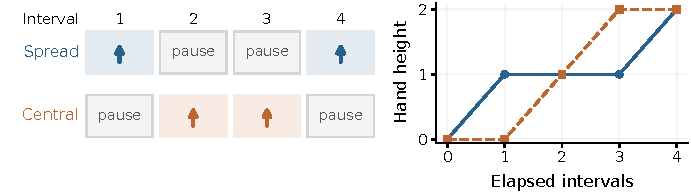
\includegraphics[width=.78\linewidth]{evidence/natops/movement_schedules.pdf}
\caption{Two four-step schedules on \([0,1]\) with identical initial height
\(0\), final height \(2\), and mean height \(1\) (\cite[Fig.~1]{mainpaper}).
The spread schedule \(a=(1,0,0,1)\) separates its unit rises across the
interval; the central schedule \(b=(0,1,1,0)\) places them together.}
\label{fig:comp-movement}
\end{figure}

\subsection{Piecewise-linear paths, signatures, and depth-two coordinates}
\label{app:general-signature}\label{app:meanings}
We recall the classical signature and Chen identities~\cite{chen} in the
piecewise-linear setting used here.
Let \(z_0, \ldots, z_{R-1} \in \R^d\), with \(R \geq 2\), be an ordered sequence
of vectors that will serve as path increments. Accumulating prefix sums
\[
 y_0 = 0 \in \R^d, \qquad y_k = \sum_{r=0}^{k-1} z_r \quad (1 \leq k \leq R),
\]
and interpolating linearly on each unit parameter interval \([r, r+1]\),
\[
 y(t) = y_r + (t - r) z_r \qquad (t \in [r, r+1],\ 0 \leq r < R),
\]
defines a continuous piecewise-linear path \(y:[0, R] \to \R^d\) with derivative
\(\dot y(t) = z_r\) on \((r, r+1)\).

\begin{definition}[Truncated path signature]\label{def:signature}
For an integer truncation depth \(m \geq 1\), the \emph{signature} of the
piecewise-linear path \(y:[0,R]\to\R^d\) through depth \(m\) is the collection
of iterated integrals
\begin{equation}\label{eq:app-general-signature}
 S_{\leq m}(y) = \bigl(1, S^1(y), \ldots, S^m(y)\bigr), \qquad
 S^{i_1 \cdots i_k}(y) = \int_{0 < t_1 < \cdots < t_k < R}
 dy^{i_1}_{t_1} \cdots dy^{i_k}_{t_k},
\end{equation}
where \(S^k(y) \in (\R^d)^{\otimes k}\) has entries \(S^{i_1 \cdots i_k}(y)\) for
\(1 \leq i_1, \ldots, i_k \leq d\).
\end{definition}

Because \(y\) is piecewise smooth, the Riemann--Stieltjes integrals
in~\eqref{eq:app-general-signature} reduce to ordinary Riemann integrals and
are invariant under orientation-preserving reparametrizations of \([0,R]\). For a
single linear step \(v \in \R^d\) traversed at constant velocity over a unit
interval, the ordered \(k\)-simplex \(\{0 < t_1 < \cdots < t_k < 1\}\) has
volume \(1/k!\), so the segment's truncated signature is the truncated tensor
exponential \(\exp_\otimes(v) = \sum_{k=0}^m v^{\otimes k} / k!\). By Chen's
identity, concatenating the \(R\) linear segments multiplies their truncated
tensor exponentials in chronological order.

Specializing to depth \(m=2\), each step \(z_r\) has signature
\((1, z_r, \tfrac12 z_r \otimes z_r)\), and inductively applying Chen's identity
across \(r = 0, \ldots, R-1\) yields explicit discrete formulas for the
first-level vector \(s = S^1(y) \in \R^d\) and second-level matrix
\(B = S^2(y) \in \R^{d \times d}\):
\begin{equation}\label{eq:app-depth-two}
 s = \sum_{r=0}^{R-1} z_r, \qquad
 B = \sum_{0 \leq r < t < R} z_r \otimes z_t
   + \frac{1}{2}\sum_{r=0}^{R-1} z_r \otimes z_r, \qquad
 J = \frac{1}{2}(B - B^\top)
   = \frac{1}{2}\sum_{0 \leq r < t < R} (z_r \otimes z_t - z_t \otimes z_r).
\end{equation}
The endpoint \(s\) records total net displacement. Adding~\eqref{eq:app-depth-two}
to its transpose gives the shuffle relation \(B + B^\top = s s^\top\), which
splits \(B\) into a symmetric endpoint product and an alternating part:
\[
 B_{ij} = \frac{1}{2} s_i s_j + J_{ij}.
\]
Geometrically, for each coordinate pair \(i < j\), \(J_{ij}\) is the L\'evy
signed area swept out in the \((y^i, y^j)\)-plane by the path closed with the
straight chord from \((y^i_R, y^j_R) = (s_i, s_j)\) back to the origin: a step
of size \(\alpha\) along axis \(i\) followed by a step of size \(\beta\) along
axis \(j\) encloses a triangle of signed area \(+\alpha\beta/2\). Together, the
\(d\) endpoints \(s_i\) and the \(\binom{d}{2}\) upper-triangular signed areas
\(J_{ij}\) (\(1 \leq i < j \leq d\)) form the \emph{depth-two logsignature} of
\(y\), capturing all order-sensitive information present at depth two.

We can now verify directly why ordinary depth-two coordinates fail to separate
the two schedules in Figure~\ref{fig:comp-movement}. A scalar height path
(\(d=1\)) has only an endpoint \(s_1 = 2\) and no off-diagonal area. Appending a
uniform clock \(T(t) = t\) on \([0,1]\) supplies timing through two-channel
increments \(\tilde z_r = (1/4, z_r) \in \R^2\). Evaluating~\eqref{eq:app-depth-two}
on both \(a = (1, 0, 0, 1)\) and \(b = (0, 1, 1, 0)\) gives the common endpoint
\(s = (1, 2)\) and the time--height signed area
\[
 J_{Tx} = \frac{1}{2}\sum_{0 \leq r < t < 4}
          \Bigl(\frac{1}{4} z_t - \frac{1}{4} z_r\Bigr)
        = \frac{1}{8}\sum_{r=0}^{3} (2r - 3) z_r = 0,
\]
because both schedules are palindromic (\(z_{3-r} = z_r\)). Consequently, both
clocked paths have the identical depth-two signature matrix
\(B = \begin{psmallmatrix} 1/2 & 1 \\ 1 & 2 \end{psmallmatrix}\): symmetric
rearrangements of rises around the midpoint cancel in \(J_{Tx}\).

\subsection{The Pascal increment lift and pairwise separation}
\label{app:movement}
Rather than relying on higher-depth iterated integrals against a single linear
clock, we can make step position visible before accumulating the path by
attaching polynomially weighted copies directly to each increment.

\begin{definition}[Pascal increment lift and Pascal-coded signature]
\label{def:pascal-lift}
Let \(z_0, \ldots, z_{R-1} \in \R^C\) with \(R \geq 2\), and choose an integer
copy count \(1 \leq P \leq R\). Define the normalized Pascal weights, lifted
increments, and accumulated vertices by
\begin{equation}\label{eq:app-pascal}
 b_p(r) = \frac{\binom{r}{p}}{\binom{R-1}{p}}, \qquad
 v_r = \bigl(b_p(r) z_r\bigr)_{p=0}^{P-1} \in \R^{PC}, \qquad
 y_k = \sum_{r < k} v_r \quad (0 \leq k \leq R),
\end{equation}
where \(\binom{r}{p} = 0\) for integers \(0 \leq r < p\), and \(y_0 = 0\). Writing
\(c_p\) for copy \(p \in \{0, \ldots, P-1\}\) of input channel
\(c \in \{1, \ldots, C\}\), the coordinate \(v_r^{c_p}\) equals \(b_p(r) z_r^c\).
Interpolating the vertices \(y_0, \ldots, y_R\) linearly on unit intervals defines
the lifted path \(y:[0,R]\to\R^{PC}\). Its ordinary truncated signature
\(S_{\leq m}(y)\) is the \emph{Pascal-coded signature} of \(z\) at copy count
\(P\) and depth \(m\).
\end{definition}

Two structural properties of Definition~\ref{def:pascal-lift} deserve emphasis.
First, the weights \(b_p(r)\) multiply the \emph{increments} \(z_r\), not the
accumulated positions \(x_r = \sum_{j < r} z_j\). Multiplying positions by
\(b_p(r)\) and then taking differences would inject terms proportional to
\(\bigl(b_p(r+1) - b_p(r)\bigr) x_r\) into the path increments, mixing step
changes with running totals; Definition~\ref{def:pascal-lift} instead combines
position-weighted increments~\cite{fruits} with piecewise-linear signature
accumulation~\cite{generalised}. Second, the two integers \(P\) and \(m\) govern
independent aspects of the representation: \(b_0(r) = 1\) embeds the unweighted
increment path \(x\) into the \(p=0\) coordinate block (so projecting
\(S_{\leq m}(y)\) onto the \(p=0\) channels recovers \(S_{\leq m}(x)\)),
\(b_1(r) = r/(R-1) = u_r\) adds linear position weights in \([0,1]\), and
increasing \(P\) nests higher polynomial degrees within single steps, whereas
increasing \(m\) lengthens chronologically ordered products across steps.

For scalar increments \(z=(z_r)_{r=0}^{R-1}\), take \(C=1\) and \(P=2\).
We label the lifted coordinates by copy number \(0,1\), so
\[
 v_r=(v_r^0,v_r^1)=(z_r,u_r z_r)\in\R^2.
\]
Coordinate \(0\) is the original copy and coordinate \(1\) is the
position-weighted copy. Accumulating \(v_r\) gives a two-dimensional path
\(y=(y^0,y^1)\). Its signed area in the \((y^0,y^1)\)-plane, closed by the
endpoint chord, is \(J_{01}\), as in the main paper. The indices \(0,1\)
label coordinates, while \(r,t\) label steps. Applying~\eqref{eq:app-depth-two} gives
\begin{equation}\label{eq:app-separation}
 J_{01} = \frac{1}{2}\sum_{0 \leq r < t < R} (z_r \cdot u_t z_t - u_r z_r \cdot z_t)
        = \frac{1}{2}\sum_{0 \leq r < t < R} (u_t - u_r) z_r z_t.
\end{equation}
Because \(u_t - u_r = (t - r)/(R-1) > 0\) whenever \(r < t\), every pair of
same-sign increments contributes half its product weighted by the normalized
index separation between the two steps. When increments take both signs,
positive and negative pairs can cancel, so \(J_{01}\) measures net weighted pair
separation rather than recovering individual inter-event delays. Note also that
within-step terms (\(r = t\)) vanish identically from~\eqref{eq:app-separation},
because each lifted step \((1, u_r) z_r\) moves along a straight ray in the
lifted plane and sweeps out zero area.

\begin{example}[Separating the two hand-movement schedules at depth two]
\label{ex:two-rises}
The scalar paths in Figure~\ref{fig:comp-movement} have spread increments
\(a = (1, 0, 0, 1)\) and central increments \(b = (0, 1, 1, 0)\).
Here \(R=4\), \(P=2\), and the scalar weights \(u_r=r/(R-1)\) satisfy
\((u_0,u_1,u_2,u_3)=(0,\tfrac13,\tfrac23,1)\).
For \(z=a\) or \(z=b\), the increments \(v_r=(z_r,u_r z_r)\) define the
two-dimensional coded path with coordinates \(0\) and \(1\). Both
schedules still share the coded endpoint
\[
 s(a) = \Bigl(1 + 1,\ 0\cdot 1 + 1\cdot 1\Bigr) = (2, 1), \qquad
 s(b) = \Bigl(1 + 1,\ \frac{1}{3}\cdot 1 + \frac{2}{3}\cdot 1\Bigr) = (2, 1),
\]
reflecting their common total rise and common center of rise. (If the uniform
clock \(\Delta T_r = 1/4\) is also included and lifted in copy-major order
\((T_0, x_0, T_1, x_1)\), both schedules likewise share the four-coordinate
endpoint \((1, 2, \tfrac12, 1)\).) However, each schedule has a single nonzero
pair \(r < t\) with \(z_r = z_t = 1\), so~\eqref{eq:app-separation} yields
distinct within-channel coded areas:
\[
 J_{01}(a) = \frac{1}{2}(1 - 0)\cdot 1\cdot 1 = \frac{1}{2}, \qquad
 J_{01}(b) = \frac{1}{2}\Bigl(\frac{2}{3} - \frac{1}{3}\Bigr)\cdot 1\cdot 1
           = \frac{1}{6}.
\]
Thus a linear readout on depth-two logsignature coordinates separates \(a\) from
\(b\) using the two lifted spatial channels \((y^0, y^1)\)---the same channel
count as the uncoded clocked path \((T, x)\) whose depth-two coordinates
coincided. The separation arises because \((y^0, y^1)\) pairs height increments
against each other across time, whereas \(J_{Tx}\) in \((T, x)\) pairs each
height increment only against the uniform clock.
\end{example}

\subsection{Linear readouts and channel-interaction graphs}
Understanding how coded coordinates feed a linear classifier requires
distinguishing information content from linear span. By \(B = J + \tfrac12 s s^\top\)
and \(J = \tfrac12(B - B^\top)\), the tensor pair \((s, B)\) and logsignature pair
\((s, J)\) determine one another bijectively. However, a linear functional of
\((s, B)\) has direct access to all quadratic endpoint products \(s_i s_j\),
whereas a linear functional of \((s, J)\) does not. Notice also that \(B\) alone
cannot replace \((s, B)\): because \(B\) is homogeneous of degree two in the
increments, negating an entire path (\(v_r \mapsto -v_r\)) leaves \(B\)
unchanged while reversing \(s\).

This distinction appears concretely when comparing two input channels
\(c, e \in \{1, \ldots, C\}\) under the two-copy lift \(u_r = r/(R-1)\). Write
\(c_0, c_1\) and \(e_0, e_1\) for their constant and linearly weighted copies.
The directed cross-channel separation sum
\[
 Q_{ce} = \sum_{0 \leq r < t < R} (u_t - u_r) z_r^c z_t^e
        = B_{c_0 e_1} - B_{c_1 e_0}
\]
is an exact linear combination of depth-two tensor coordinates (their within-step
terms \(\tfrac12 u_r z_r^c z_r^e\) cancel in the difference). Rewriting \(B\) in
terms of \((s, J)\) splits \(Q_{ce}\) into a linear area combination plus a
quadratic endpoint determinant:
\[
 Q_{ce} = (J_{c_0 e_1} + J_{e_0 c_1})
        + \frac{1}{2}(s_{c_0} s_{e_1} - s_{c_1} s_{e_0}).
\]
In logsignature coordinates, the two natural linear combinations of cross-copy
areas instead isolate symmetric pair separation and midpoint-weighted order:
\begin{align*}
 J_{c_0 e_1} + J_{e_0 c_1}
   &= \frac{1}{2}\sum_{0 \leq r < t < R} (u_t - u_r)(z_r^c z_t^e + z_r^e z_t^c), \\
 J_{c_0 e_1} - J_{e_0 c_1}
   &= \frac{1}{2}\sum_{0 \leq r < t < R} (u_r + u_t)(z_r^c z_t^e - z_r^e z_t^c).
\end{align*}
When \(c = e\), the endpoint determinant \(s_{c_0} s_{c_1} - s_{c_1} s_{c_0}\)
vanishes identically and \(Q_{cc} = 2 J_{c_0 c_1}\), which is why single-channel
pair separation belongs linearly to the depth-two logsignature.

Exposing multichannel interactions through \(P\) copies carries a quadratic
dimension cost. Lifting \(C\) channels to \(d = PC\) channels produces
\(\sum_{k=1}^m d^k\) non-scalar tensor coordinates through depth \(m\)
(\(d + d^2 = PC + P^2 C^2\) at depth two) and \(d + \binom{d}{2}\) depth-two
logsignature coordinates. When kinematic or sensor structure suggests retaining
cross-channel areas only across a specified graph \(E \subseteq \binom{\{1,\ldots,C\}}{2}\)
of unordered distinct channel pairs, keeping all \(PC\) endpoints, all
\(\binom{P}{2}\) same-channel cross-copy areas per input channel, and all \(P^2\)
copy-pair areas for each edge \(\{c, e\} \in E\) yields the nominal dimension
\begin{equation}\label{eq:graph-dimension}
 d_{\mathrm{graph}}(C, P, E) = PC + P^2 |E| + C\binom{P}{2}.
\end{equation}
Taking \(|E| = \binom{C}{2}\) recovers \(PC + \binom{PC}{2}\); taking \(E = \emptyset\)
retains only endpoints and single-channel separation areas, matching the sum of
\(C\) independent scalar depth-two logsignatures,
\(C\bigl(P + \binom{P}{2}\bigr)\). More generally, partitioning the channels into
disjoint groups and computing a depth-two logsignature within each group omits
cross-group areas while retaining all within-group interactions. All such
formulas count nominal coordinates; when an observation convention introduces
constant channels (such as a unit clock or unit-sum spectrum), the number of
nonconstant or linearly independent features is smaller.

\subsection{What increments represent: movement, posture, and rhythm}
\label{app:spectral-meaning}
The algebraic formulas~\eqref{eq:app-depth-two}--\eqref{eq:app-separation} are
agnostic to the physical origin of \(z_r\). Choosing how raw measurements map to
increments determines whether endpoints and areas summarize spatial gestures,
static postures, or oscillatory spectra:

\paragraph{1. Anchored displacements for spatial trajectories.}
In landmark-based action recognition~\cite{yang,generalised}, given sequential
coordinates \(x_0, \ldots, x_R \in \R^C\), taking first differences
\(z_r = x_{r+1} - x_r\) makes the path sensitive to movement while discarding any
global translation \(x_r \mapsto x_r + c\). When absolute starting pose also
distinguishes classes, prepending an initial step \(z_{\mathrm{init}} = x_0 - 0\)
from a fixed coordinate origin anchors the path: the unweighted endpoint becomes
the final pose \(x_R\), and signed areas between \(z_{\mathrm{init}}\) and
subsequent displacements record motion relative to the initial configuration.
Section~\ref{app:natops} applies this convention to 3D body-landmark gestures.

\paragraph{2. Scaled sensor readings for persistent posture levels.}
For body-worn accelerometers and gyroscopes, differencing \(a_{r+1} - a_r\)
annihilates constant gravitational orientation and merges static postures such
as sitting, standing, and lying down. Standardizing sensor readings \(a_r \in \R^C\)
using training-set statistics \emph{without} centering individual windows and
setting
\[
 z_r = \frac{a_r}{R} \qquad (0 \leq r < R)
\]
instead builds a cumulative path whose constant-copy endpoint
\(s_0 = R^{-1}\sum_{r=0}^{R-1} a_r\) is the window mean. Static posture levels
remain directly accessible, while higher Pascal copies \(b_p(r) z_r\) supply
temporal trends and ordered cross-axis interactions across the window
(Sections~\ref{app:har} and~\ref{app:additional}).

\paragraph{3. Frequency-ordered power shares for spectral shape and spread.}
Sustained rhythmic activities such as walking or cycling concentrate variance in
narrow frequency bands. To describe this concentration independently of the
phases of the Fourier coefficients, we apply the Pascal lift to power ordered
along the frequency axis~\cite{mainpaper}. Let
\(e_0, \ldots, e_{K-1} \geq 0\) be the one-sided Fourier power of a real scalar
signal at \(K \geq 2\) strictly increasing frequencies \(f_0 < \cdots < f_{K-1}\).
Whenever total power \(E = \sum_{k=0}^{K-1} e_k\) is positive, the normalized
shares \(p_k = e_k / E\) satisfy \(p_k \geq 0\) and \(\sum_{k=0}^{K-1} p_k = 1\),
defining the law of a discrete random frequency \(F\) with \(\Pr(F = f_k) = p_k\).

Here, energy refers to squared signal amplitude. Under the Parseval normalization
used in Section~\ref{app:har}, a scalar window \(x_0,\ldots,x_{n-1}\) has total
power \(E=n^{-1}\sum_r x_r^2\): the average squared reading. Squaring counts
both positive and negative readings as signal strength. For a fixed preprocessed
window, doubling every reading quadruples \(E\) but leaves the shares \(p_k\)
unchanged. The zero-frequency power \(e_0=\bar x^2\) records the constant
(mean) component.

Treating the scalar shares \(z_k = p_k\) as increments ordered by frequency bin
\(k = 0, \ldots, K-1\) and lifting with monomial frequency weights
\((1, f_k, f_k^2)\) gives coded endpoints equal to the spectral moments
\[
 s_0 = \sum_{k=0}^{K-1} p_k = 1, \qquad
 s_1 = \sum_{k=0}^{K-1} f_k p_k = \E[F], \qquad
 s_2 = \sum_{k=0}^{K-1} f_k^2 p_k = \E[F^2],
\]
namely unit mass, the spectral centroid, and the noncentral second moment.
The spectral centroid is the energy-weighted average frequency. For example,
energy shares \(3/4\) at \(2\,\mathrm{Hz}\) and \(1/4\) at \(6\,\mathrm{Hz}\)
give a centroid of \(3\,\mathrm{Hz}\). It describes where the power is centered,
which need not be a frequency present in the signal. The main paper uses the
normalized grid \(u_k=k/(K-1)\), so its centroid \(\sum_k u_kp_k\) lies in
\([0,1]\); for equally spaced frequencies starting at zero, multiplying by
\(f_{K-1}\) converts it to the original frequency units.

For an independent copy \(G\) drawn from the same distribution \(\Pr(G = f_l) = p_l\),
the pair-separation identity~\eqref{eq:app-separation} gives the constant--linear
signed area a clean probabilistic meaning:
\begin{equation}\label{eq:spectral-separation}
 J^{(1,f)}_{01} = \frac{1}{2}\sum_{0 \leq k < l < K} (f_l - f_k) p_k p_l
                = \frac{1}{4}\sum_{k=0}^{K-1}\sum_{l=0}^{K-1} |f_l - f_k| p_k p_l
                = \frac{1}{4}\E|F - G|,
\end{equation}
since each unordered pair \(\{k, l\}\) with \(k \neq l\) appears twice in the
double sum and diagonal terms vanish. Thus \(4 J^{(1,f)}_{01}\) is the classical
\emph{Gini mean difference} of the normalized power spectrum, using the full
mean-absolute-difference normalization. Its area interpretation is the
classical Gini--Lorenz relation~\cite[Sec.~2]{gini}. Shifting every frequency by a
constant leaves \(J^{(1,f)}_{01}\) unchanged, while splitting a unit spectral line
at \(f_*\) into two equal sidebands of mass \(1/2\) at \(f_* - \delta\) and
\(f_* + \delta\) keeps the centroid \(\E[F] = f_*\) fixed and increases
\(J^{(1,f)}_{01}\) from \(0\) to \(\delta/4\). (This captures spread beyond the
centroid without implying statistical independence of \(s_1\) and \(J^{(1,f)}_{01}\)
across signals.)

Because normalizing by \(E\) removes overall signal strength, a spectral shape
logsignature must be paired with separate amplitude summaries whenever vibration
intensity matters. Writing \(a_k = \sqrt{e_k}\) for the unnormalized bin
amplitudes, retaining their mean \(\bar a = K^{-1}\sum_{k=0}^{K-1} a_k\) and
population standard deviation \(\sigma_a = \sqrt{K^{-1}\sum_{k=0}^{K-1}(a_k - \bar a)^2}\)
preserves total spectral power through the exact identity
\[
 E = \sum_{k=0}^{K-1} a_k^2 = K(\bar a^2 + \sigma_a^2),
\]
which equals the time-domain mean square under the Parseval-normalized one-sided
Fourier transform specified in Section~\ref{app:har}.
